\documentclass[conference]{IEEEtran}

% ── Encoding & Language (engine-agnostic) ──────────────────────────
\usepackage{iftex}
\ifPDFTeX
  \usepackage[utf8]{inputenc}
  \usepackage[T5]{fontenc}
\else
  \usepackage{fontspec}
  \defaultfontfeatures{Ligatures=TeX}
  \setmainfont{Latin Modern Roman}
\fi
\usepackage[vietnamese,english]{babel}

\usepackage{amsmath,amssymb}
\usepackage{bm}
\usepackage{graphicx}
\graphicspath{{figures/}}
\usepackage{booktabs}
\usepackage{multirow}
\usepackage{array}
\usepackage{float}
\usepackage[hidelinks]{hyperref}
\usepackage{caption}
\usepackage{xcolor}
\usepackage{enumitem}
\usepackage[backend=biber, style=ieee, sorting=none]{biblatex}
\addbibresource{references.bib}

\newcommand{\sys}{\textit{InternHub}}
\newcommand{\auc}{ROC-AUC}
\newcommand{\prauc}{PR-AUC}

% ══════════════════════════════════════════════════════════════════
\begin{document}

\title{InternHub: Hệ Thống Phân Loại và Gợi Ý Phỏng Vấn IT\\ Cá Nhân Hóa Dựa Trên Knowledge Tracing}

\author{
  \IEEEauthorblockN{Mai Dương Hải Đăng}
  \IEEEauthorblockA{Trường ĐH Công nghệ Thông tin\\ ĐHQG-HCM\\ 24520253@gm.uit.edu.vn}
  \and
  \IEEEauthorblockN{Tạ Gia Khiêm}
  \IEEEauthorblockA{Trường ĐH Công nghệ Thông tin\\ ĐHQG-HCM\\ 24520805@gm.uit.edu.vn}
  \and
  \IEEEauthorblockN{Nguyễn Sỹ Huỳnh}
  \IEEEauthorblockA{Trường ĐH Công nghệ Thông tin\\ ĐHQG-HCM\\ 24520716@gm.uit.edu.vn}
  \and
  \IEEEauthorblockN{Nguyễn Ngọc Nam}
  \IEEEauthorblockA{Trường ĐH Công nghệ Thông tin\\ ĐHQG-HCM\\ 24521114@gm.uit.edu.vn}
}

\maketitle

\begin{abstract}
Khóa luận trình bày \sys{}, một hệ thống luyện phỏng vấn IT cá nhân hóa tích hợp Knowledge Tracing (KT) cho ba vai trò dữ liệu phổ biến: Data Analyst (DA), Data Scientist (DS) và Data Engineer (DE). Hệ thống giải quyết hai hạn chế của các nền tảng hiện nay: thiếu cá nhân hóa theo năng lực và không theo dõi quỹ đạo kiến thức của người học. Nhóm xây dựng question bank đa dạng (5 loại câu hỏi, 17 Knowledge Components) bằng pipeline lai giữa thu thập nguồn công khai và sinh tự động bằng mô hình ngôn ngữ lớn (LLM) kèm kiểm định chất lượng; đồng thời thiết kế pipeline mô phỏng dựa trên Item Response Theory (IRT) để tạo dữ liệu huấn luyện KT (1.000 người dùng ảo, $\sim$40.000 tương tác). Ba họ mô hình KT---BKT, DKT, SAKT---được huấn luyện và so sánh, gồm biến thể \textit{quality label} liên tục. Trên tập kiểm tra, mọi mô hình KT vượt baseline ($\auc \approx 0.68$ so với $0.50$); DKT-Quality đạt $\prauc = 0.907$ và RMSE $= 0.355$, tốt nhất trong nhóm neural. Một cơ chế cập nhật năng lực thời gian thực kết hợp dự đoán KT (70\%) với trung bình trượt mũ EMA (30\%) được tích hợp vào engine gợi ý theo chiến lược \textit{zone of proximal development} và bài kiểm tra thích nghi hai giai đoạn. Toàn bộ được hiện thực thành ứng dụng web hoàn chỉnh (React + FastAPI + Streamlit) với chấm điểm tự động bằng LLM và cơ chế chấm dự phòng cục bộ.
\end{abstract}

\begin{IEEEkeywords}
Knowledge Tracing, Deep Knowledge Tracing, Item Response Theory, hệ thống gợi ý, kiểm tra thích nghi, luyện phỏng vấn IT.
\end{IEEEkeywords}

% ══════════════════════════════════════════════════════════════════
\section{Giới Thiệu}
\label{sec:intro}

Thị trường tuyển dụng nhân lực công nghệ thông tin tại Việt Nam và trên thế giới đang chứng kiến sự cạnh tranh ngày càng gay gắt. Theo khảo sát của TopDev~\cite{topdev2024}, hơn 70\% ứng viên IT tại Việt Nam thừa nhận chưa chuẩn bị đủ kỹ năng kỹ thuật cần thiết trước các vòng phỏng vấn, trong khi phần lớn các nền tảng luyện phỏng vấn hiện có (LeetCode, HackerRank, Pramp) chủ yếu tập trung vào lập trình thuật toán, thiếu nội dung dành riêng cho ba vai trò dữ liệu phổ biến: Data Analyst (DA), Data Scientist (DS) và Data Engineer (DE).

Hai thách thức cốt lõi tồn tại với các nền tảng hiện tại. Thứ nhất, \textbf{thiếu cá nhân hóa theo năng lực}: hầu hết hệ thống cung cấp câu hỏi theo cách tĩnh, không phản ánh được trình độ thực tế của từng ứng viên---người có kinh nghiệm phải làm lại các câu quá dễ, trong khi người mới bắt đầu nản lòng với câu hỏi ngoài tầm. Vấn đề này tương ứng với khái niệm \textit{zone of proximal development} trong tâm lý học giáo dục~\cite{vygotsky1978mind}: câu hỏi hiệu quả nhất là câu hơi khó hơn năng lực hiện tại của người học một chút. Thứ hai, \textbf{không theo dõi được quỹ đạo kiến thức}: hệ thống hiện có không duy trì và cập nhật trạng thái kiến thức của người học theo thời gian, nên sau mỗi phiên luyện tập không biết người dùng đã tiến bộ ở điểm nào, còn yếu kỹ năng nào, và câu hỏi tiếp theo nên đi theo hướng nào.

Knowledge Tracing (KT)~\cite{corbett1994knowledge} là hướng giải quyết được nghiên cứu nhiều trong lĩnh vực Educational Data Mining~\cite{romero2010educational,baker2010data}, giúp mô hình hóa và dự đoán trạng thái kiến thức của người học qua lịch sử tương tác. Các mô hình KT từ Bayesian Knowledge Tracing~\cite{corbett1994knowledge} đến Deep Knowledge Tracing~\cite{piech2015deep} và Self-Attentive Knowledge Tracing~\cite{pandey2019self} đã chứng minh hiệu quả trong môi trường học thuật. Tuy nhiên, việc áp dụng KT cho bài toán luyện phỏng vấn IT---với đặc thù câu hỏi mở, chấm điểm tự động bằng LLM~\cite{team2023gemini} và nhiều loại câu hỏi (lý thuyết, coding, tình huống)---vẫn là một bài toán mở.

Khóa luận đặt ra bốn \textbf{mục tiêu}: (1) xây dựng bộ dữ liệu luyện KT phù hợp cho bài toán phỏng vấn IT; (2) huấn luyện và so sánh ba họ mô hình KT (BKT, DKT, SAKT) với biến thể nhãn nhị phân và quality label liên tục; (3) xây dựng engine gợi ý dựa trên KT theo chiến lược ZPD, có hỗ trợ kiểm tra thích nghi hai giai đoạn; (4) tích hợp vào ứng dụng web hoàn chỉnh với chấm điểm LLM và fallback cục bộ.

\textbf{Phạm vi.} Trong phạm vi: ba vai trò DA/DS/DE; 17 Knowledge Components (DA 5, DS 7, DE 5); năm loại câu hỏi (MC\_SINGLE, TRUE\_FALSE, FILL\_BLANK, THEORY, CODING); dữ liệu KT mô phỏng gồm 1.000 người dùng, $\sim$40.000 tương tác. Ngoài phạm vi: dữ liệu người dùng thật, triển khai production quy mô lớn, và A/B testing so với hệ thống thương mại.

\textbf{Đóng góp chính.} (1) Một pipeline xây dựng dữ liệu phỏng vấn IT tổng hợp, có thể tái sử dụng cho các bài toán KT nghề nghiệp khác; (2) biến thể DKT-Quality dùng nhãn chất lượng liên tục, cải thiện RMSE và \prauc{}; (3) cơ chế blend KT(70\%) + EMA(30\%) với ngưỡng kích hoạt 3 tương tác, giải quyết cold-start; (4) hệ thống luyện phỏng vấn IT end-to-end tích hợp KT, kiểm tra thích nghi và chấm điểm LLM trong một codebase chạy local.

% ══════════════════════════════════════════════════════════════════
\section{Công Trình Liên Quan}
\label{sec:related}

\textbf{Knowledge Tracing.} Từ BKT~\cite{corbett1994knowledge}, các mô hình KT đã phát triển qua DKT~\cite{piech2015deep}, DKVMN~\cite{zhang2017dynamic}, AKT~\cite{ghosh2020context}, và gần đây là các mô hình Transformer-based như SAINT~\cite{choi2020towards}. SAKT~\cite{pandey2019self} là mô hình attention đầu tiên đơn giản và hiệu quả, dựa trên cơ chế self-attention~\cite{vaswani2017attention}. Một số hướng mở rộng tích hợp nội dung bài tập (EKT~\cite{liu2019ekt}) hoặc cải thiện tính nhất quán của dự đoán DKT~\cite{yeung2018addressing}. Gần đây, một số nghiên cứu khảo sát khả năng của LLM trong giáo dục và đánh giá~\cite{liu2023llm,brown2020language}.

\textbf{Hệ thống học thích nghi.} Knewton~\cite{ferreira2017knewton} và ASSISTments~\cite{heffernan2014assistments} sử dụng KT để cá nhân hóa lộ trình học. Tuy nhiên, các hệ thống này tập trung vào môi trường học thuật, chưa có ứng dụng cụ thể cho phỏng vấn IT.

\textbf{Hệ thống gợi ý.} Các kỹ thuật như matrix factorization~\cite{koren2009matrix} và neural collaborative filtering~\cite{he2017neural} phổ biến trong recsys nói chung. \sys{} khác biệt ở chỗ kết hợp KT với chiến lược ZPD thay vì chỉ dựa trên độ tương đồng giữa người dùng.

\textbf{Hệ thống luyện phỏng vấn.} Các nền tảng như LeetCode, HackerRank cung cấp bài tập lập trình nhưng thiếu cơ chế theo dõi kiến thức có cấu trúc. \sys{} khác biệt ở chỗ tích hợp KT với question bank đa dạng (lý thuyết, thực hành, coding) cho ba vai trò DA/DS/DE, đồng thời sử dụng LLM để chấm điểm tự động.

% ══════════════════════════════════════════════════════════════════
\section{Cơ Sở Lý Thuyết}
\label{sec:theory}

\subsection{Knowledge Tracing}
Cho một chuỗi tương tác $\{(q_1,r_1),\ldots,(q_t,r_t)\}$ trong đó $q_t$ là câu hỏi tại thời điểm $t$ và $r_t$ là kết quả, mục tiêu của KT là dự đoán xác suất trả lời đúng câu hỏi tiếp theo $p(r_{t+1}=1\mid q_{t+1}, q_{1:t}, r_{1:t})$. Trong \sys{}, KT được áp dụng để theo dõi năng lực của ứng viên trên 17 Knowledge Components (KC) thuộc ba vai trò.

\subsubsection{Bayesian Knowledge Tracing (BKT)}
BKT~\cite{corbett1994knowledge} mô hình hóa từng KC như một chuỗi Markov ẩn (HMM) với hai trạng thái: \textit{chưa thành thạo} và \textit{thành thạo}, đặc trưng bởi bốn tham số cho mỗi KC: $P(L_0)$ (xác suất thành thạo ban đầu), $P(T)$ (chuyển trạng thái), $P(S)$ (slip---trả lời sai dù thành thạo), $P(G)$ (guess---trả lời đúng dù chưa thành thạo). Xác suất trả lời đúng tại bước $t$:
\begin{equation}
P(r_t=1)=P(L_t)(1-P(S))+(1-P(L_t))P(G).
\end{equation}
Sau mỗi quan sát, trạng thái thành thạo được cập nhật theo Bayes:
\begin{equation}
P(L_t\mid r_t=1)=\frac{P(L_t)(1-P(S))}{P(r_t=1)},
\end{equation}
\begin{equation}
P(L_{t+1})=P(L_t\mid r_t)+(1-P(L_t\mid r_t))P(T).
\end{equation}
Tham số BKT được ước lượng bằng EM hoặc tối ưu trực tiếp L-BFGS-B trên log-likelihood. Ưu điểm: diễn giải cao, hiệu quả trên dữ liệu nhỏ; hạn chế: giả định KC độc lập.

\subsubsection{Deep Knowledge Tracing (DKT)}
DKT~\cite{piech2015deep} thay mô hình xác suất bằng mạng LSTM~\cite{hochreiter1997long}, cho phép học biểu diễn ẩn phong phú hơn:
\begin{equation}
\mathbf{h}_t=\text{LSTM}(\mathbf{x}_t,\mathbf{h}_{t-1}),\quad \hat{y}_{t+1}=\sigma(\mathbf{W}\mathbf{h}_t+\mathbf{b}).
\end{equation}
\sys{} mở rộng DKT với \textbf{quality label}: thay nhãn nhị phân $r_t\in\{0,1\}$ bằng điểm chất lượng liên tục $r_t\in[0,1]$ phản ánh mức độ thành thạo, chuyển hàm mất mát từ Binary Cross-Entropy sang MSE:
\begin{equation}
\mathcal{L}_{\text{quality}}=\frac{1}{T}\sum_{t=1}^{T}(r_t-\hat{y}_t)^2.
\end{equation}

\subsubsection{Self-Attentive Knowledge Tracing (SAKT)}
SAKT~\cite{pandey2019self} thay kiến trúc hồi quy bằng self-attention~\cite{vaswani2017attention}, học mối liên hệ trực tiếp giữa các KC liên quan trong lịch sử. Attention score giữa câu $q_t$ và bước lịch sử $s$:
\begin{equation}
a_{t,s}=\frac{(\mathbf{e}_{q_t}\mathbf{W}^Q)(\mathbf{m}_s\mathbf{W}^K)^\top}{\sqrt{d}}.
\end{equation}
Ưu điểm: song song hóa (không tuần tự như LSTM) và diễn giải được attention weight.

\subsection{Item Response Theory}
IRT~\cite{embretson2000item,lord1980applications} mô hình hóa quan hệ giữa năng lực người học $\theta$ và xác suất trả lời đúng câu hỏi $i$. Mô hình 3PL dùng trong simulation:
\begin{equation}
P(r=1\mid\theta,a_i,b_i,c_i)=c_i+(1-c_i)\frac{1}{1+e^{-a_i(\theta-b_i)}},
\end{equation}
với $a_i$ là độ phân biệt, $b_i$ là độ khó, $c_i$ là xác suất đoán. Trong \sys{}, $b$ ánh xạ từ EASY/MEDIUM/HARD thành $\{0.30,0.55,0.80\}$.

\subsection{Cập nhật năng lực thời gian thực: EMA và Blend}
Mô hình KT cho dự đoán tốt khi đã đủ lịch sử, nhưng kém ổn định ở giai đoạn cold-start. \sys{} kết hợp KT với Exponential Moving Average (EMA). Với mỗi KC, sau điểm $s_t\in[0,1]$:
\begin{equation}
\theta^{\text{EMA}}_t=\alpha s_t+(1-\alpha)\theta^{\text{EMA}}_{t-1},\quad \alpha=0.35.
\end{equation}
EMA luôn chạy ngay từ tương tác đầu tiên. Khi lịch sử đạt tối thiểu 3 tương tác, dự đoán KT được blend với EMA:
\begin{equation}
\hat{\theta}_t=\lambda\,\theta^{\text{KT}}_t+(1-\lambda)\,\theta^{\text{EMA}}_t,\quad \lambda=0.70.
\label{eq:blend}
\end{equation}
KT (trọng số trội) nắm bắt động lực chuỗi và quan hệ giữa các KC; EMA (30\%) ổn định hóa dự đoán, chống dao động khi gặp chuỗi nhiễu. Hằng số $\lambda$ và ngưỡng 3 tương tác được giữ nhất quán giữa backend và frontend để con số hiển thị đồng bộ trên toàn hệ thống.

% ══════════════════════════════════════════════════════════════════
\section{Xây Dựng Dữ Liệu}
\label{sec:data}

\subsection{Thu thập và kiểm định Question Bank}
Khác với phần lớn nghiên cứu KT chỉ dùng dataset có sẵn, khóa luận tự xây dựng question bank phỏng vấn IT qua một quy trình lai bốn giai đoạn. \textbf{Thu thập}: câu hỏi được scraping từ nhiều kho phỏng vấn mở (bộ DE của Obenner, bộ SQL của LearningZone, các bộ DS/DA cộng đồng), có trích dẫn nguồn, rồi ánh xạ sơ bộ về vai trò và nhóm kỹ năng. \textbf{Sinh tự động}: để tăng độ phủ các KC còn thiếu, một pipeline đa mô hình LLM được dùng---một mô hình sinh câu hỏi mới theo từng KC và mức độ, một mô hình mạnh hơn tạo đáp án tham chiếu và các \textit{evaluation points}, một mô hình \textit{judge} chấm chất lượng và một mô hình \textit{enhancer} tinh chỉnh diễn đạt~\cite{team2023gemini,brown2020language}. \textbf{Kiểm định chất lượng}: mỗi câu đi qua kiểm tra schema, đối chiếu nội dung bằng RAG để phát hiện câu sai sự thật, và review thủ công trên mẫu ngẫu nhiên. \textbf{Chuẩn hóa}: ánh xạ các tag chi tiết (ví dụ \texttt{SQL\_WINDOW\_FUNCTION}) về 17 KC chuẩn qua bảng tra gồm 82 ánh xạ. Snapshot dùng cho thực nghiệm KT gồm 1.578 câu (17 KC, 3 mức độ); sau khi tiếp tục thu thập và sinh bổ sung, question bank của ứng dụng triển khai mở rộng lên 2.122 câu.

\begin{figure}[t]
  \centering
  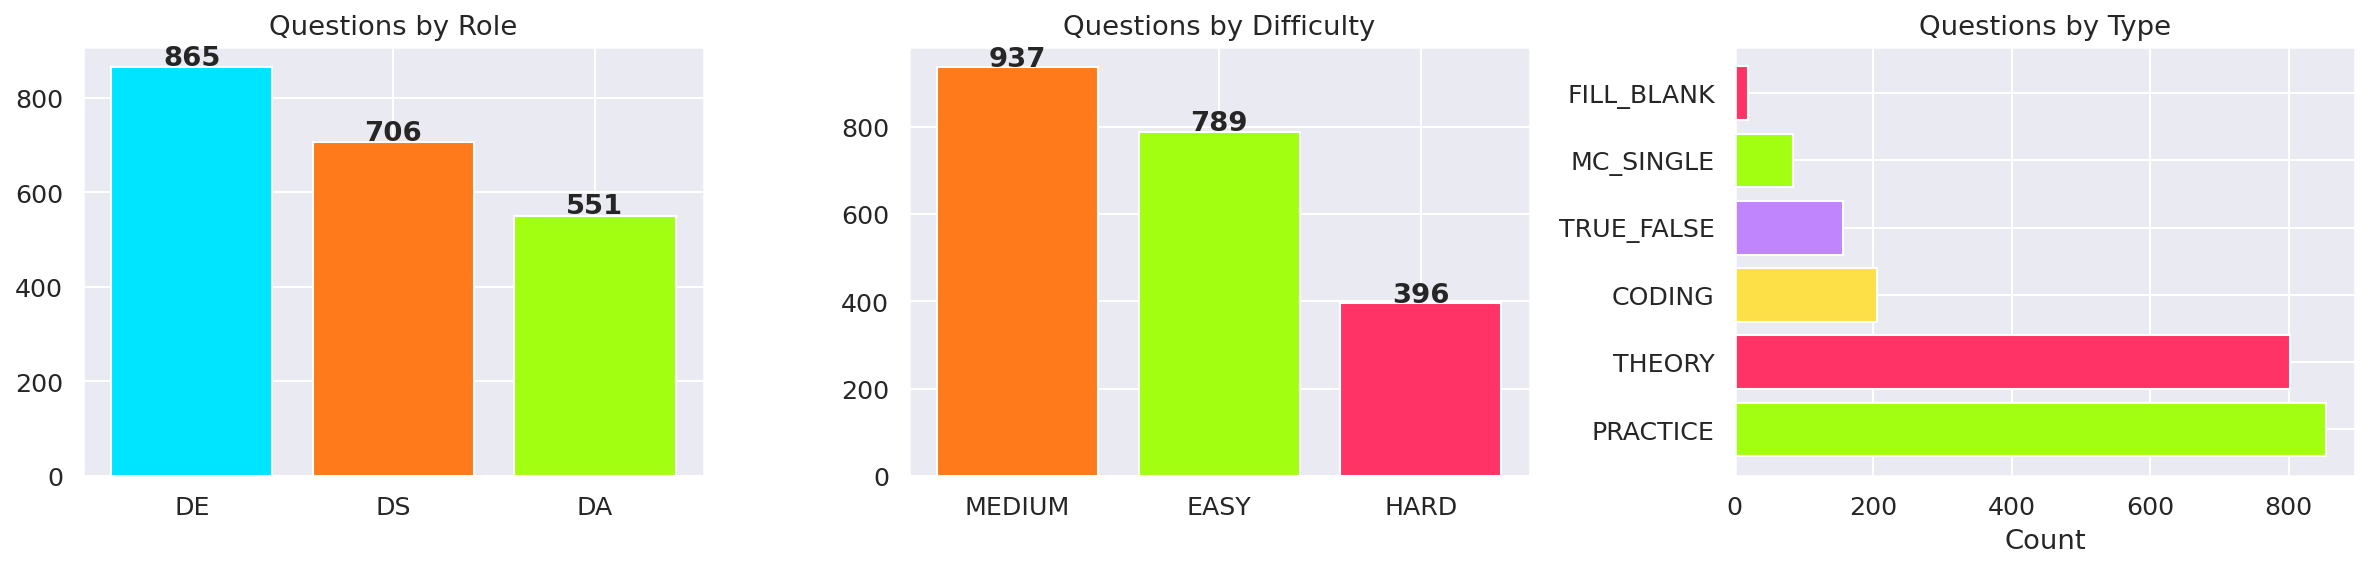
\includegraphics[width=0.95\columnwidth]{eda_qbank_distribution.png}
  \caption{Phân bố câu hỏi theo vai trò và mức độ khó trong question bank.}
  \label{fig:qbank}
\end{figure}

\subsection{Mô phỏng tương tác bằng IRT}
Do thiếu dữ liệu thực từ người dùng thật, nhóm sử dụng pipeline mô phỏng ba bước. \textbf{Bước 1}: sinh 1.000 người dùng ảo với skill vector theo phân phối correlated Gaussian, phản ánh tương quan thực tế giữa các competency (ví dụ DA có $r(\text{SQL},\text{Analytics})\approx 0.55$; DS có $r(\text{Algorithm},\text{Evaluation})\approx 0.70$). \textbf{Bước 2}: với mỗi user, sinh chuỗi tương tác dựa trên IRT, $P(\text{correct})=\sigma((\theta-b)\times 6)$. \textbf{Bước 3}: chấm theo bậc bằng power-based graded response, $P(Q{=}2)=p^{\alpha}$, $P(Q{=}0)=(1-p)^{\alpha}$ với $\alpha=2.0$, và cập nhật skill: $\theta\mathrel{+}=\eta(1-\theta)$ khi đúng, $\theta\mathrel{-}=\gamma\theta$ khi sai, với $\eta=0.08$, $\gamma=0.002$, seed 42.

\begin{table}[t]
  \centering
  \caption{Thống kê bộ dữ liệu mô phỏng}
  \label{tab:dataset}
  \begin{tabular}{lr}
    \toprule
    \textbf{Thuộc tính} & \textbf{Giá trị} \\
    \midrule
    Người dùng & 1.000 (DA 334 / DS 333 / DE 333) \\
    Câu hỏi (snapshot KT) & 1.578 \\
    Knowledge Components & 17 \\
    Tổng tương tác & 40.140 (TB 40,1/user) \\
    Train & 700 users / 28.164 tương tác \\
    Validation & 150 users / 5.911 tương tác \\
    Test & 150 users / 6.065 tương tác \\
    Pass rate ($Q\geq 1$) & 82,5\% \\
    \bottomrule
  \end{tabular}
\end{table}

\subsection{Kiểm tra toàn vẹn dữ liệu}
Trước huấn luyện, bộ dữ liệu được kiểm tra qua bảy tiêu chí: (1) không rò rỉ user giữa train và test; (2) phân phối nhãn train (82,7\%) $\approx$ test (82,2\%), chênh $<1\%$; (3) độ dài chuỗi đồng đều (trung bình 40 bước); (4) drift tần suất KC---2/17 KC có drift $>3\%$; (5) class imbalance 82,5\% positive nên cần dùng \prauc{} thay vì chỉ \auc{}; (6) phân phối quality hợp lý; (7) 100\% người dùng có cold-start vector.

% ══════════════════════════════════════════════════════════════════
\section{Phân Tích Khám Phá Dữ Liệu}
\label{sec:eda}

\textbf{Phân tích người dùng.} Phân bổ người dùng đều theo vai trò (DA 334, DS 333, DE 333). Sau khi phân loại lại dựa trên skill vector thực, phân phối trình độ là beginner 40,9\%, intermediate 53,2\%, advanced 5,9\%---lệch so với mục tiêu thiết kế (35/50/15\%) do nhiều user advanced bị reclassify về intermediate khi mean skill nằm trong khoảng $[0.40, 0.70]$. Heatmap skill vector cho thấy tương quan dương rõ giữa các KC trong cùng vai trò.

\textbf{Phân tích question bank.} Question bank có phân bố khá đồng đều giữa ba vai trò, mỗi vai trò khoảng 500--550 câu; trong mỗi vai trò, câu MEDIUM chiếm tỷ lệ lớn nhất---phù hợp với thực tế phỏng vấn. Độ phủ theo KC có chênh lệch: các KC phổ biến như \texttt{SQL\_DATABASE} (DA) và \texttt{ALGORITHM\_THEORY} (DS) có nhiều câu hơn.

\textbf{Phân tích tương tác.} Phân phối quality score nhất quán với thiết kế IRT: $Q{=}2\approx 62\%$, $Q{=}1\approx 20\%$, $Q{=}0\approx 18\%$ (Hình~\ref{fig:quality}). Phân tầng theo độ khó xác nhận câu EASY có tỷ lệ $Q{=}2$ cao hơn rõ, câu HARD có $Q{=}0$ cao hơn; câu MEDIUM cân bằng nhất---vùng có độ phân biệt cao nhất trong IRT. Heatmap pass rate theo competency cho thấy các KC phức tạp như \texttt{DEEP\_LEARNING} và \texttt{NLP} của DS có pass rate thấp nhất.

\begin{figure}[t]
  \centering
  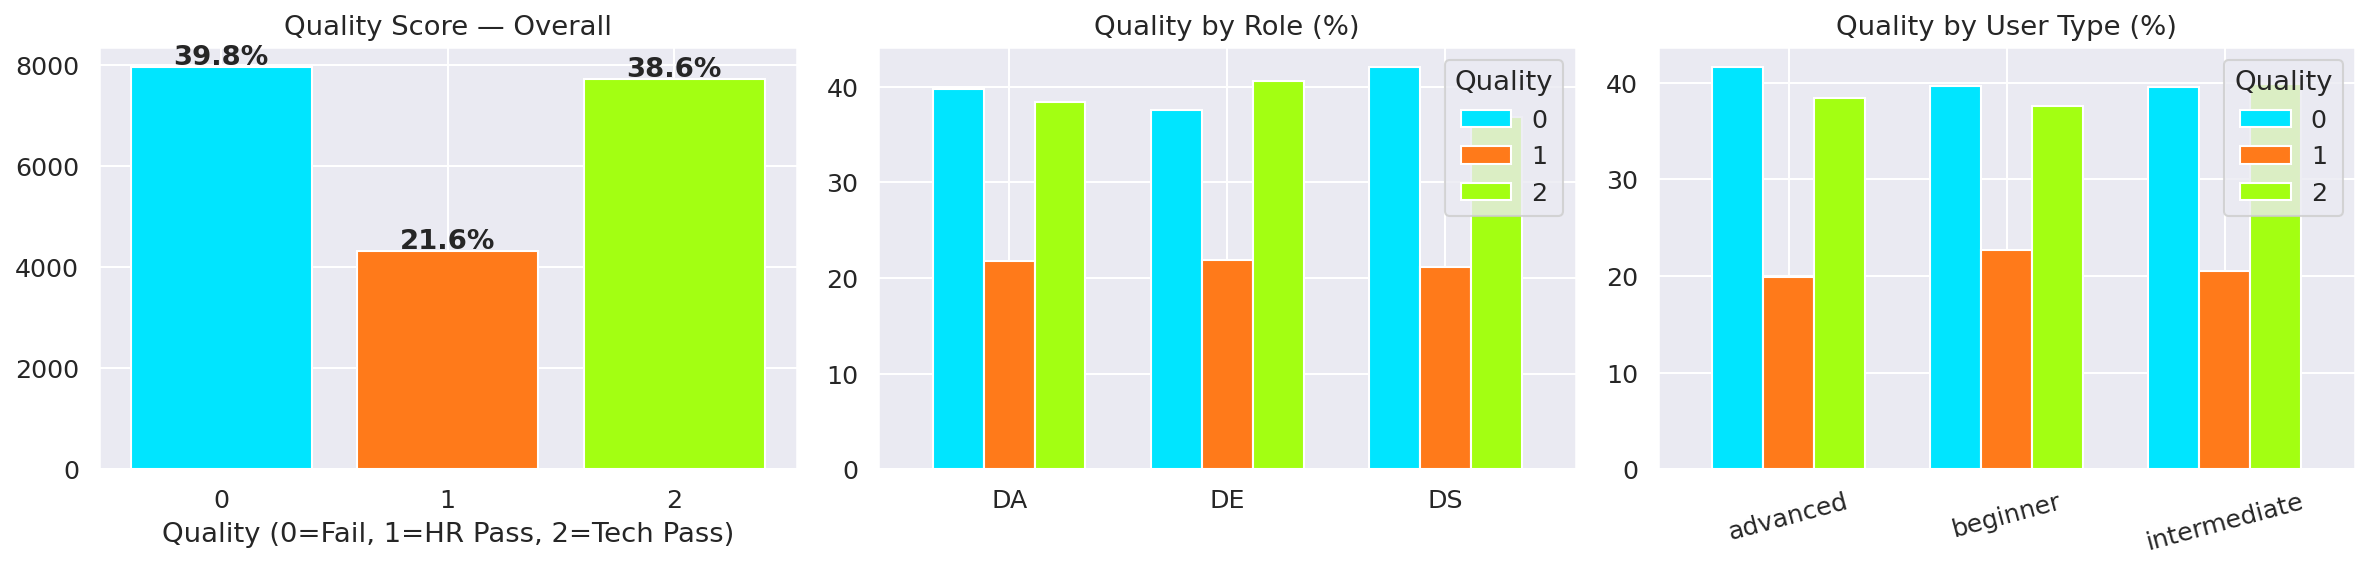
\includegraphics[width=0.85\columnwidth]{eda_quality_distribution.png}
  \caption{Phân phối quality score (0 = Fail, 1 = Pass HR, 2 = Pass Tech).}
  \label{fig:quality}
\end{figure}

\textbf{Sparsity và learning dynamics.} Ma trận tương tác user--KC có cấu trúc block-diagonal do mỗi user chỉ trả lời câu thuộc vai trò của mình, dẫn đến sparsity $\approx 77\%$ trên toàn không gian KC nhưng chỉ $\approx 15$--$20\%$ trong từng vai trò---đủ để BKT hoạt động ổn định. Toàn bộ user có đúng 40 tương tác do pool câu mỗi vai trò sau bộ lọc competency bị cap ở mức $\approx$40 câu. Learning curve tăng đơn điệu theo thứ tự câu (Hình~\ref{fig:lc}), xác nhận động lực học đúng theo $\Delta\theta=\eta(1-\theta)$: skill tăng nhanh hơn khi còn thấp. Phân tầng theo trình độ cho thấy nhóm beginner có tốc độ tăng skill tuyệt đối lớn nhất, nhóm advanced có hiệu ứng trần. Phân tích confidence bias cho hệ số tương quan $r(\text{self-rating},\text{skill})\approx 0.72$; nhóm beginner có xu hướng tự tin thái quá (overconfidence).

\begin{figure}[t]
  \centering
  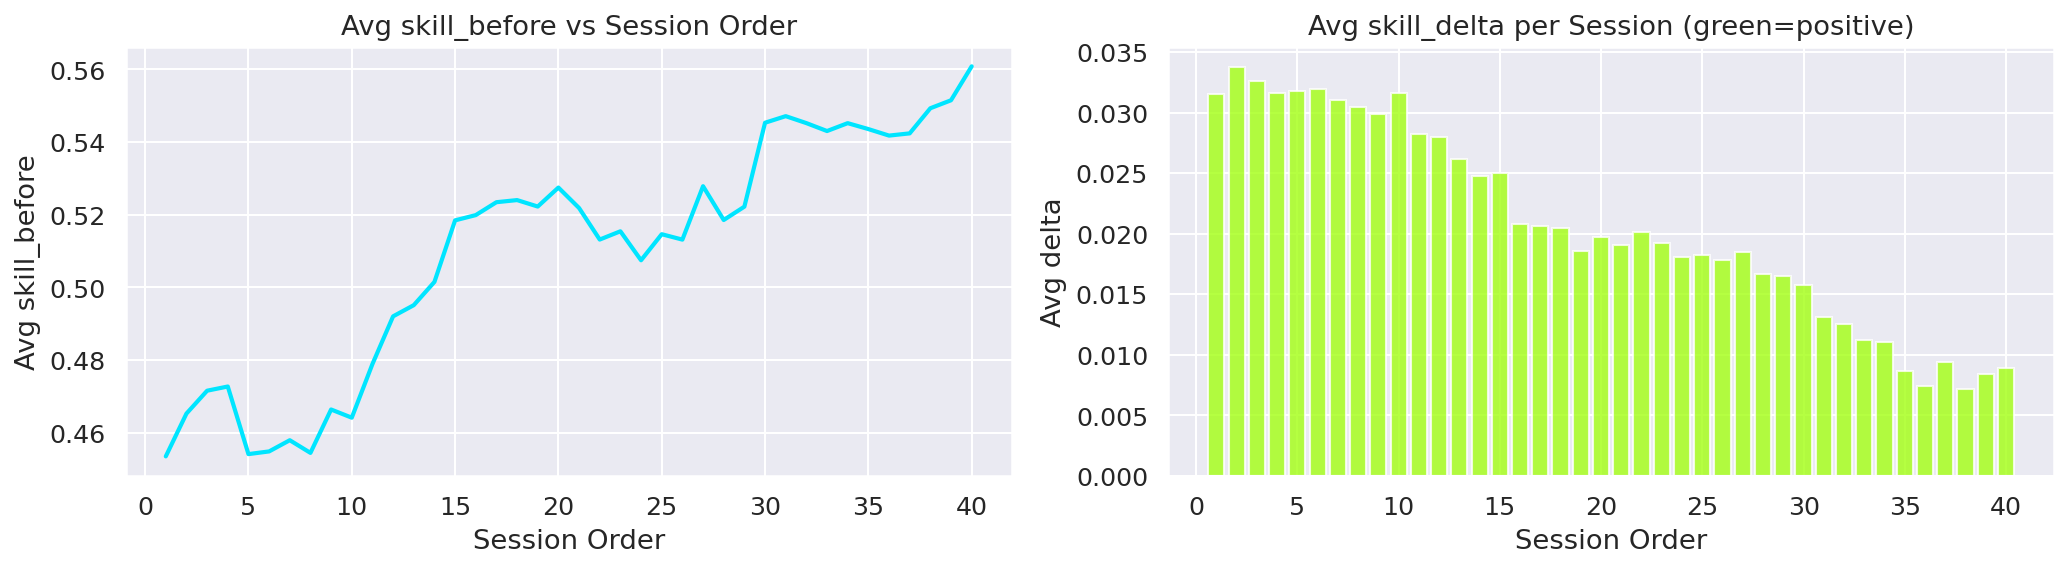
\includegraphics[width=0.85\columnwidth]{eda_learning_curve.png}
  \caption{Learning curve: skill trung bình theo vị trí trong chuỗi tương tác.}
  \label{fig:lc}
\end{figure}

% ══════════════════════════════════════════════════════════════════
\section{Thực Nghiệm và Kết Quả}
\label{sec:exp}

\subsection{Môi trường và cấu hình}
Thực nghiệm chạy trên Kaggle Notebooks (CPU Intel Xeon 2-core 13GB RAM, GPU NVIDIA Tesla T4 16GB, PyTorch 2.6~\cite{pytorch2019}, Python 3.12, seed 42). Ablation study gồm tám cấu hình: Baseline (majority class), BKT (L-BFGS-B per KC), DKT-Binary và DKT-Quality$^\star$ ($h{=}128$, $L{=}1$, dropout $0.2$~\cite{srivastava2014dropout}, lr $10^{-3}$), SAKT-Binary và SAKT-Quality$^\star$ ($e{=}64$, $H{=}4$, $L{=}1$), DKT-Deep ($h{=}256$, $L{=}2$) và SAKT-Deep ($e{=}128$, $L{=}2$). Mô hình neural dùng batch 64, tối đa 30 epoch, early stopping patience 5.

\subsection{Độ đo}
Nhóm dùng \auc{} (phân biệt đúng/sai, không phụ thuộc ngưỡng), \prauc{} (phù hợp khi mất cân bằng lớp), \prauc{} Gain ($=\prauc_{\text{model}}-\prauc_{\text{baseline}}$, đo cải thiện thực so với đường cơ sở), RMSE, và Accuracy. Do positive rate 82,5\%, \prauc{} Gain là chỉ số so sánh chính.

\subsection{Kết quả}
Bảng~\ref{tab:results} và Hình~\ref{fig:ablation} cho thấy mọi mô hình KT vượt baseline rõ rệt: \auc{} tăng từ 0.50 lên 0.67--0.68, \prauc{} Gain đạt 0.083--0.087. Learning curves (Hình~\ref{fig:lcurves}) cho thấy các mô hình neural hội tụ ổn định trong $\sim$15--19 epoch.

\begin{table*}[t]
  \centering
  \caption{Kết quả ablation study trên tập test (150 người dùng, 6.065 tương tác)}
  \label{tab:results}
  \begin{tabular}{lrrrrrr}
    \toprule
    \textbf{Mô hình} & \textbf{\auc} & \textbf{\prauc} & \textbf{\prauc{} Gain} & \textbf{RMSE} & \textbf{Acc} & \textbf{Time (s)} \\
    \midrule
    Baseline           & 0.500 & 0.820 & 0.000 & 0.384 & 0.820 & 0.0 \\
    BKT                & \textbf{0.677} & 0.905 & 0.085 & 0.374 & 0.820 & 61.9 \\
    DKT-Binary         & 0.666 & 0.905 & 0.085 & 0.375 & 0.822 & 30.8 \\
    DKT-Quality$^\star$& 0.672 & \textbf{0.907} & \textbf{0.087} & \textbf{0.355} & 0.796 & 20.9 \\
    SAKT-Binary        & 0.668 & 0.903 & 0.083 & 0.373 & 0.822 & \textbf{11.3} \\
    SAKT-Quality$^\star$& 0.667 & 0.904 & 0.084 & 0.356 & 0.776 & 12.0 \\
    DKT-Deep           & 0.669 & 0.906 & 0.086 & 0.375 & 0.822 & 116.4 \\
    SAKT-Deep          & 0.670 & 0.906 & 0.086 & 0.373 & 0.822 & 31.4 \\
    \bottomrule
  \end{tabular}
  \\[2pt]
  \small{$^\star$: dùng quality label liên tục, tốt nhất trong nhóm neural.}
\end{table*}

\begin{figure}[t]
  \centering
  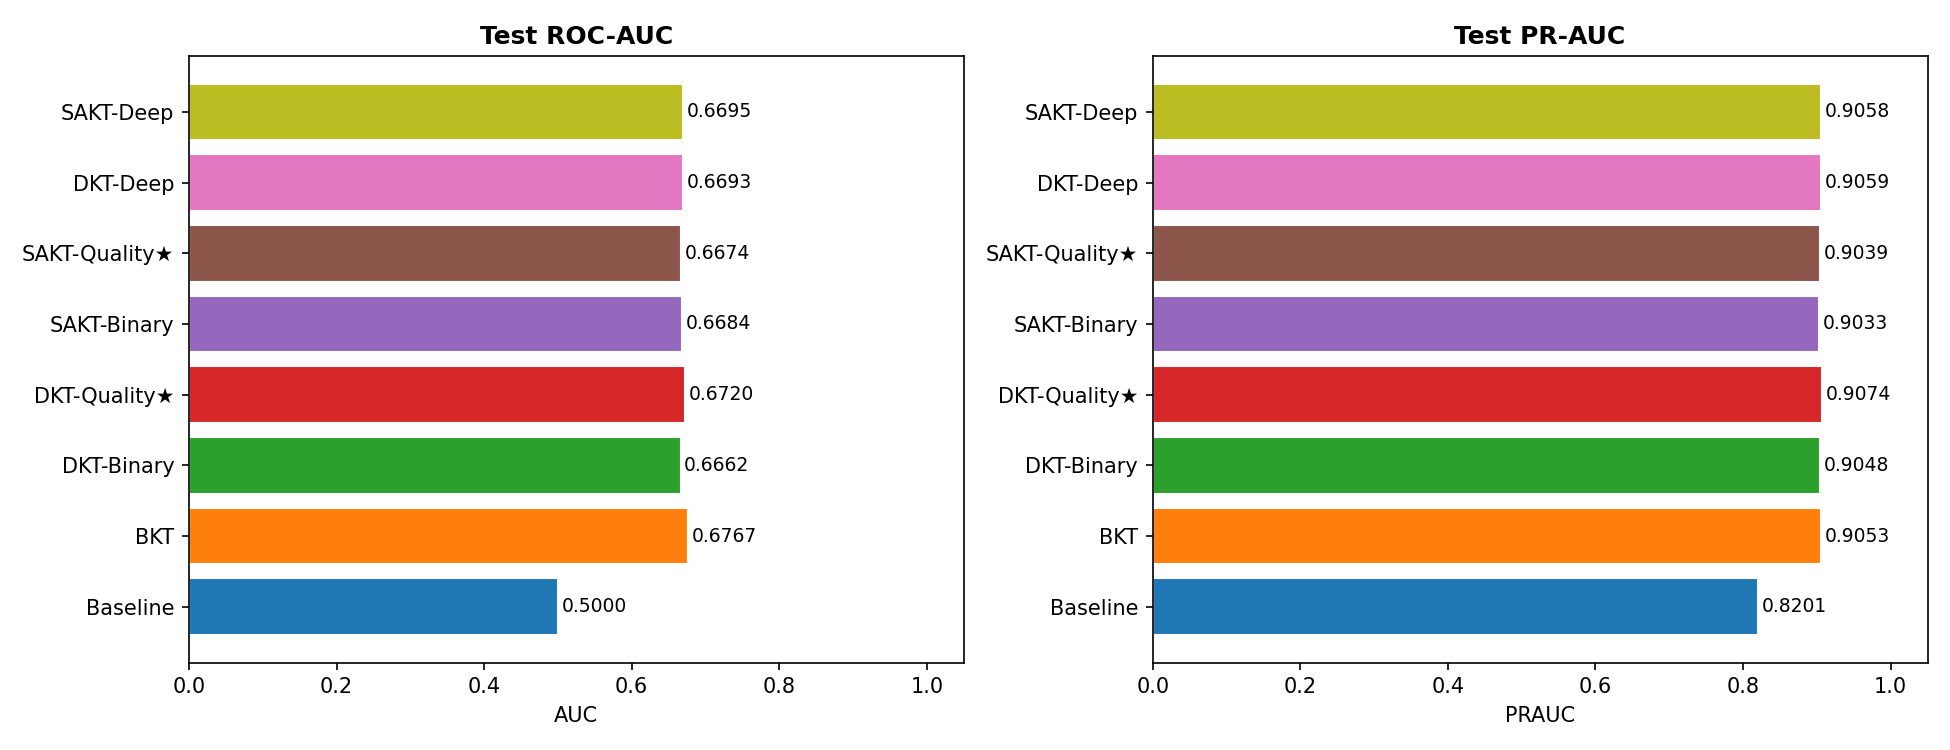
\includegraphics[width=0.95\columnwidth]{ablation_bar.png}
  \caption{So sánh \auc{} và \prauc{} của 8 cấu hình.}
  \label{fig:ablation}
\end{figure}

\begin{figure}[t]
  \centering
  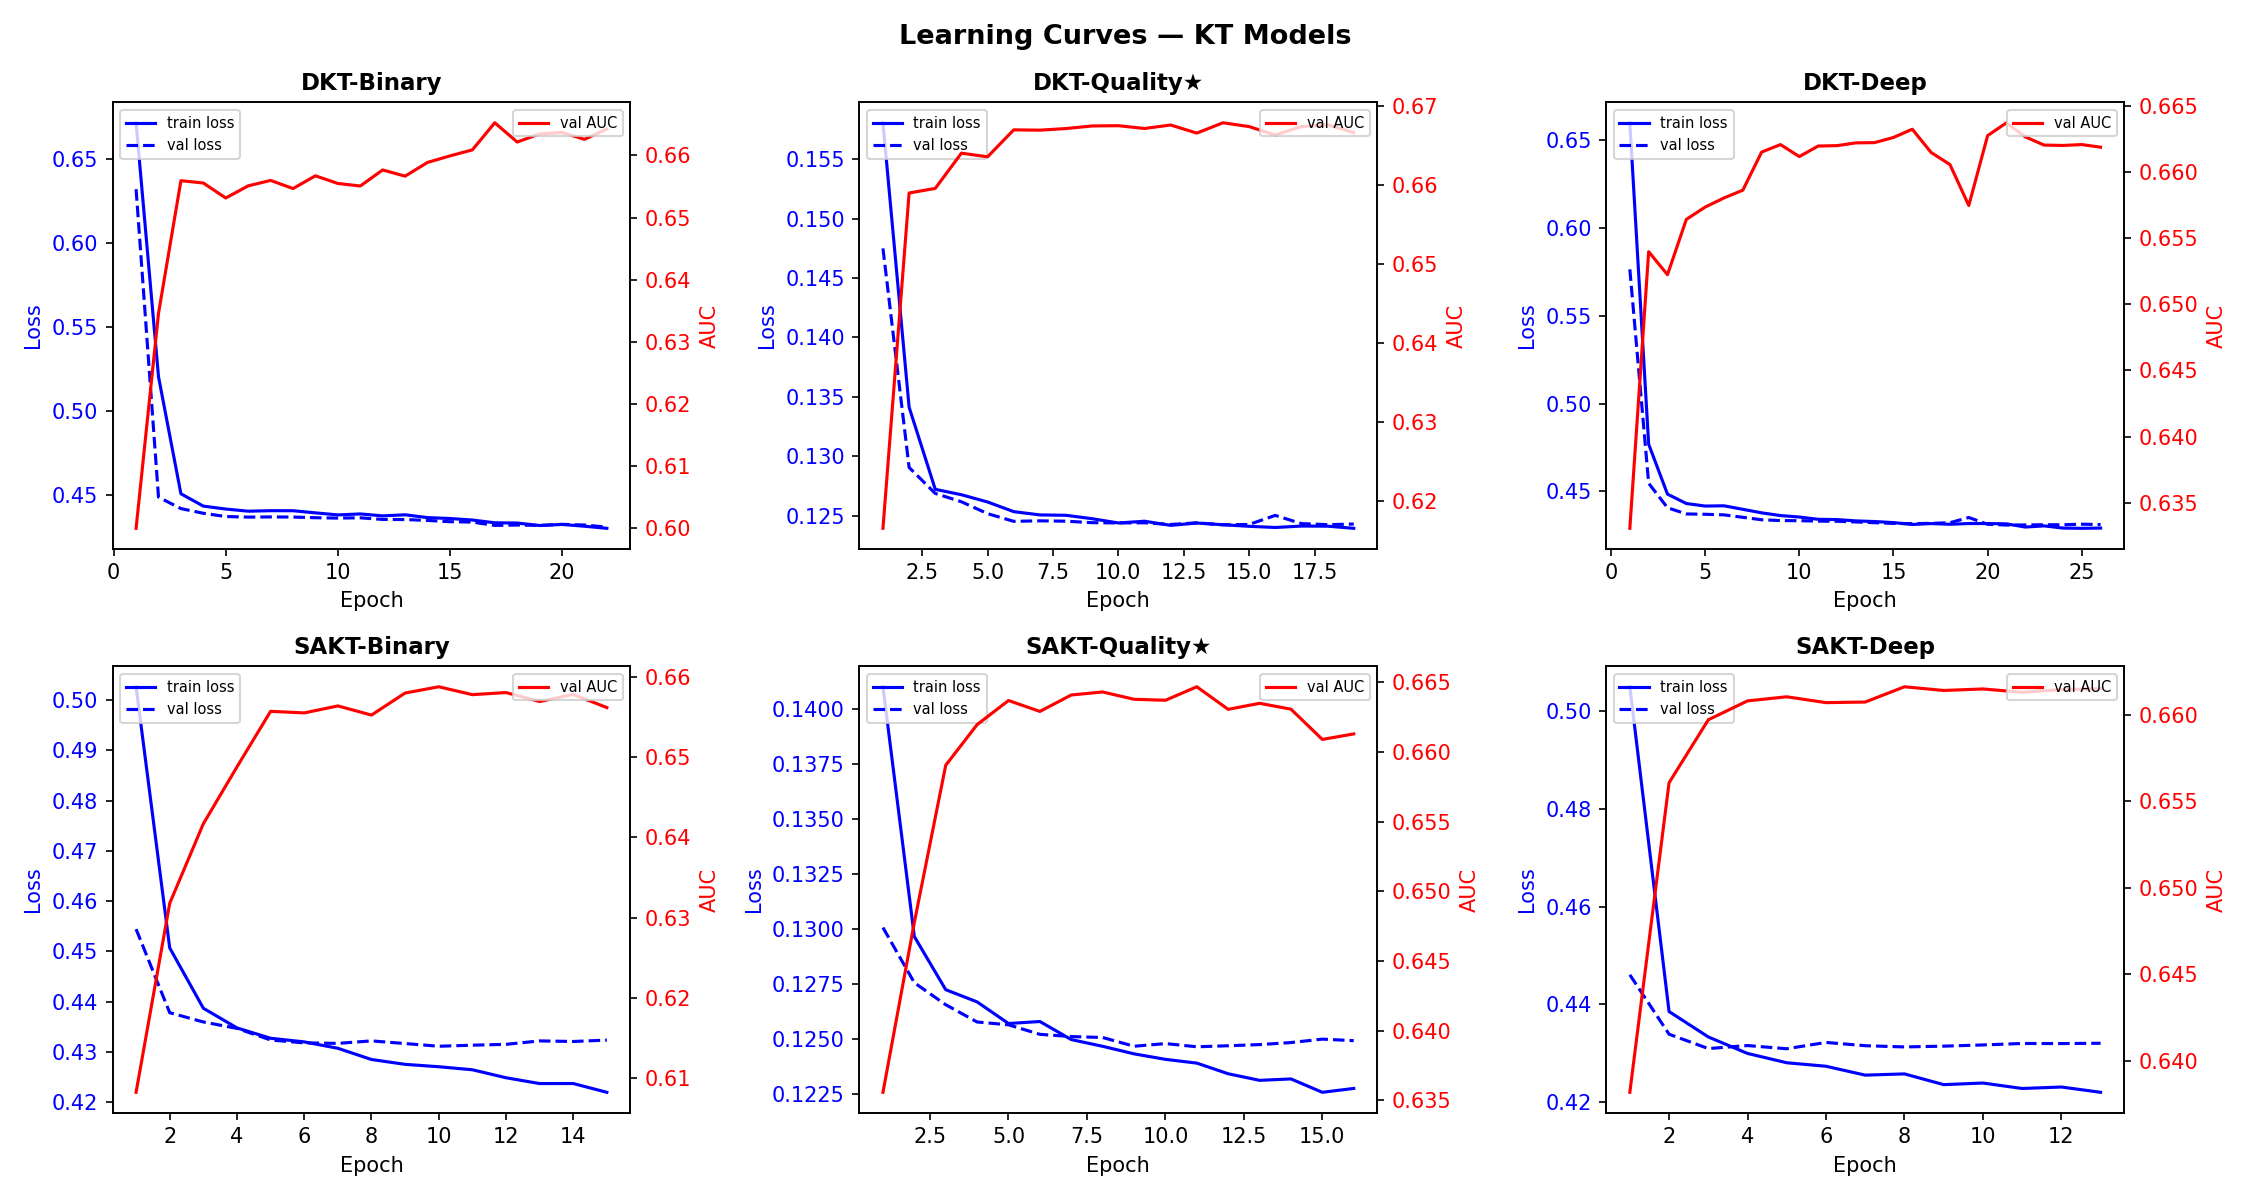
\includegraphics[width=0.95\columnwidth]{learning_curves.png}
  \caption{Learning curves của các mô hình neural (train/val loss, val \auc{}).}
  \label{fig:lcurves}
\end{figure}

\subsection{Phân tích}
\textbf{Hiệu quả KT.} Tất cả mô hình KT vượt baseline, chứng minh lịch sử tương tác mang thông tin dự đoán thực sự ngay cả với dữ liệu mô phỏng.

\textbf{Quality label.} DKT-Quality$^\star$ đạt \prauc{} cao nhất (0.907) và RMSE thấp nhất (0.355), vượt DKT-Binary (0.905, 0.375); nhãn liên tục cung cấp tín hiệu gradient phong phú hơn. Accuracy thấp hơn (0.796 so với 0.822) do tối ưu MSE thay vì cross-entropy, làm phân phối đầu ra lệch khỏi ngưỡng 0.5.

\textbf{Simulation bias.} BKT đạt \auc{} cao nhất (0.677) vì dữ liệu được sinh theo IRT---về cơ bản cùng dạng tham số per-KC với BKT, tạo lợi thế không công bằng. Trên dữ liệu thật, mô hình neural được kỳ vọng tốt hơn nhờ học được các pattern phức tạp hơn.

\textbf{Deep model.} DKT-Deep (2 LSTM layer, 256 hidden) không cải thiện đáng kể so với DKT-Binary nhưng tốn thời gian gấp gần 4 lần (116s so với 31s); SAKT-Deep tương tự. Nút thắt là kích thước dữ liệu (28K tương tác train), không phải kiến trúc.

\textbf{Hiệu quả tính toán.} SAKT-Binary có thời gian huấn luyện ngắn nhất (11s) với \auc{} cạnh tranh, nhờ khả năng song song hóa của self-attention---phù hợp cho online update.

\subsection{Phân tích sâu}
Phân tích chi tiết bổ sung cho thấy: \textit{(i) theo KC} (Hình~\ref{fig:perkc}), hiệu suất không đồng đều---KC tần suất thấp có \auc{} thấp hơn, và DKT-Quality$^\star$ vượt BKT ở phần lớn KC thuộc DS/DE; \textit{(ii) theo vị trí}, cả ba mô hình cải thiện \auc{} khi có nhiều lịch sử hơn (early $\to$ late), xác nhận giá trị của việc thu thập nhiều tương tác; \textit{(iii) theo độ khó}, câu MEDIUM có \auc{} cao nhất---vùng phân biệt cao nhất trong IRT; \textit{(iv) theo loại người dùng}, nhóm intermediate dễ dự đoán nhất do phân phối đúng/sai cân bằng; \textit{(v) cold-start}, cold-start score có tương quan dương yếu với độ chính xác per-user, xác nhận nó mang thông tin bổ sung nhưng không phải yếu tố duy nhất; \textit{(vi) phân tích lỗi} (Hình~\ref{fig:err}), mô hình thiên về dự đoán Pass do class imbalance, và phân phối điểm dự đoán phân biệt được hai nhóm nhưng có chồng lấp do nhiễu mô phỏng.

\begin{figure}[t]
  \centering
  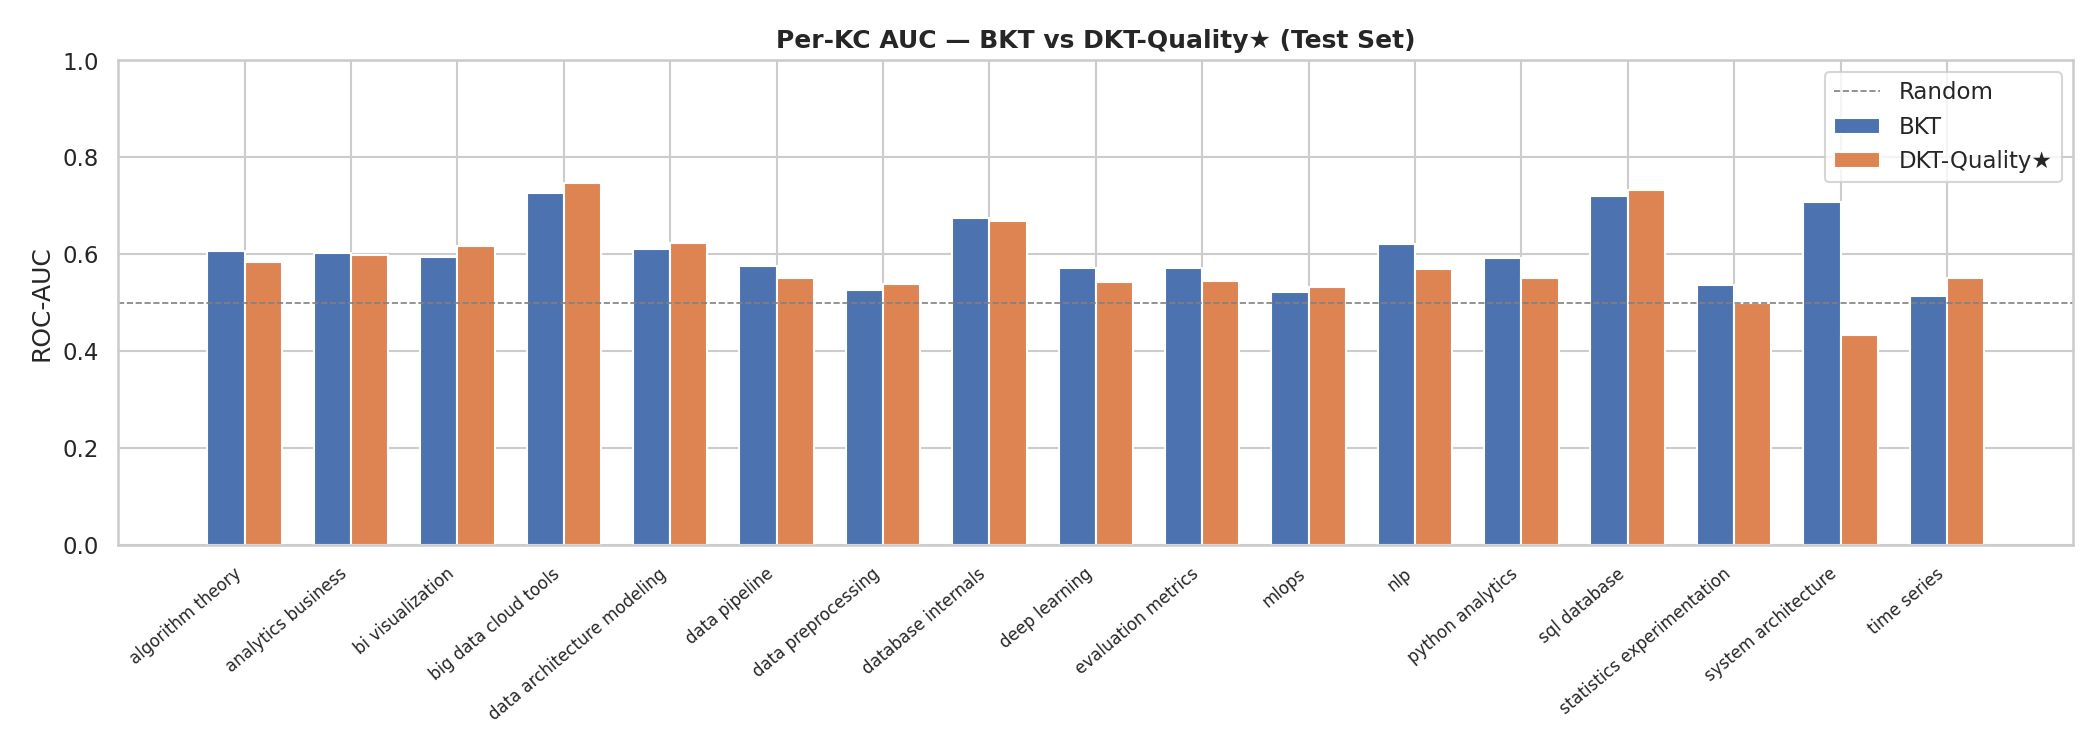
\includegraphics[width=0.95\columnwidth]{per_kc_auc.png}
  \caption{\auc{} theo từng KC: BKT vs DKT-Quality$^\star$.}
  \label{fig:perkc}
\end{figure}

\begin{figure}[t]
  \centering
  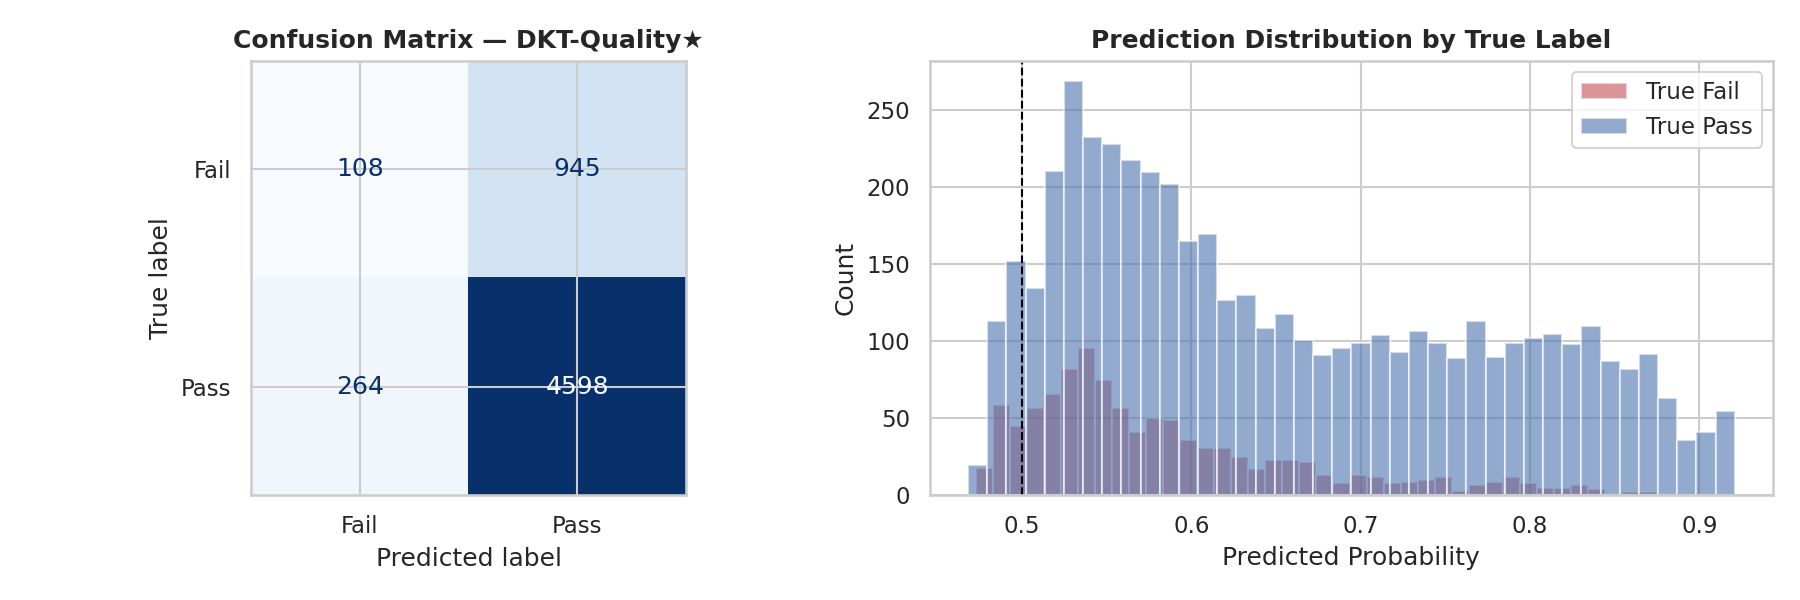
\includegraphics[width=0.95\columnwidth]{error_analysis.png}
  \caption{Confusion matrix và phân phối điểm dự đoán---DKT-Quality$^\star$.}
  \label{fig:err}
\end{figure}

\subsection{Lựa chọn mô hình}
Nhóm chọn DKT-Quality$^\star$ làm mô hình chính cho ứng dụng: output dạng $(B,T,17)$ cho phép dự đoán cả 17 KC trong một forward pass (quan trọng cho gợi ý thời gian thực), đồng thời đạt \prauc{}/RMSE tốt nhất nhóm neural và train nhanh ($\approx$21s). SAKT-Binary là lựa chọn cho online update nhanh khi cần.

% ══════════════════════════════════════════════════════════════════
\section{Thiết Kế và Hiện Thực Hệ Thống}
\label{sec:system}

\subsection{Kiến trúc ba tầng}
\sys{} được tổ chức thành ba tầng. \textbf{Tầng dữ liệu} chứa question bank, JSON schema và taxonomy 17 KC. \textbf{Tầng KT/scoring} gồm \texttt{kt\_predictor} (nạp DKT-Quality), \texttt{recommender} và \texttt{competency\_engine}. \textbf{Tầng phục vụ} gồm FastAPI~\cite{fastapi2018} (9 endpoint \texttt{/api/*}), Streamlit~\cite{streamlit2019} làm host và React SPA~\cite{react2013}. Backend (snake\_case) và frontend (camelCase) dùng quy ước đặt tên và lược đồ câu hỏi khác nhau; mọi phép chuẩn hóa được tập trung tại \textit{ranh giới} ở hai điểm: \texttt{\_map\_question()} (Python$\to$React) và \texttt{\_normalize\_question()} (React$\to$Python).

\subsection{Engine năng lực và gợi ý}
\texttt{competency\_engine} định nghĩa taxonomy 17 KC theo vai trò và bảng tra \texttt{SKILL\_GROUP\_TO\_KC} (82 ánh xạ), cùng hai ngưỡng phân loại: KC yếu nếu $\theta<0.40$, KC mạnh nếu $\theta\geq 0.70$. Engine gợi ý xếp hạng câu hỏi theo điểm tổng hợp. Khi tập trung KC yếu:
\begin{equation}
\text{score}(q)=0.65\cdot\text{weakness}+0.30\cdot\text{diff\_fit}+0.05\cdot\text{coverage},
\end{equation}
trong đó \textit{weakness}$=\max(0,0.40-\theta_{kc})/0.40$, \textit{diff\_fit} đo độ phù hợp độ khó với năng lực (chiến lược ZPD), \textit{coverage} thưởng cho phủ KC chưa mạnh. Ở chế độ thử thách, trọng số đổi thành $0.45$ readiness $+0.45$ diff\_fit $+0.10$ coverage. Khi chạy, \texttt{kt\_predictor} nạp DKT-Quality (singleton) và dự đoán mastery $\in[0.05,0.99]$; nếu lịch sử $<3$ hoặc không nạp được model thì lui về EMA thuần (graceful fallback).

\subsection{Kiểm tra thích nghi hai giai đoạn}
Phiên Diagnostic áp dụng CAT hai giai đoạn~\cite{wainer2000computerized}. \textbf{Stage 1} chọn câu phủ đều các KC của vai trò; điểm trung bình quyết định routing WEAK/MID/STRONG. \textbf{Stage 2} chọn câu chuyên sâu, ưu tiên các KC yếu nhất phát hiện ở Stage 1, độ khó điều chỉnh theo nhánh (STRONG ưu tiên ADVANCED; WEAK ưu tiên INTERMEDIATE để học). Vector năng lực cập nhật theo từng trục KC---chỉ trục được kiểm tra mới đổi; lần đánh giá đầu tiên ánh xạ trực tiếp điểm số thành giá trị KC. Điểm cuối dùng pipeline KT--EMA chung (Công thức~\eqref{eq:blend}) nên radar ở màn kết quả, Dashboard và màn KT Model đều hiển thị cùng một con số.

\subsection{Hệ thống chấm điểm}
Câu khách quan (MC\_SINGLE, TRUE\_FALSE, FILL\_BLANK) được chấm tất định phía client, không gọi LLM. Câu tự luận và coding (THEORY, PRACTICE, CODING) được chấm bằng Gemini~\cite{team2023gemini} với prompt chứa câu hỏi, đáp án tham chiếu và evaluation points. Khi Gemini lỗi (rate limit, mạng), hệ thống lui về local rubric: một evaluation point được coi là ``đạt'' khi $\geq 50\%$ từ khóa của nó xuất hiện trong câu trả lời; nếu không có eval points thì dùng độ tương đồng Jaccard từ khóa so với đáp án tham chiếu.

\subsection{Tầng phục vụ và giao diện}
Streamlit không phục vụ tốt tệp tĩnh với đúng MIME type, nên UI thực không do Streamlit phục vụ: \texttt{app.py} khởi động FastAPI ở thread nền (cổng 8000), FastAPI mount thư mục \texttt{static/} qua \texttt{StaticFiles(html=True)}; trang Streamlit chỉ là một \texttt{<iframe>}; React gọi ngược về \texttt{/api} qua \texttt{fetch}. Frontend gồm các tệp JSX nạp tuần tự bằng thẻ \texttt{<script type="text/babel">} và biên dịch ngay trên trình duyệt bằng Babel standalone---không cần npm/webpack; mọi tệp chia sẻ một global scope và dữ liệu question bank được serialize từ Python qua \texttt{window.\_\_INTERNHUB\_DATA\_\_}.

% ══════════════════════════════════════════════════════════════════
\section{Hạn Chế và Thảo Luận}
\label{sec:limit}

\textbf{Simulation bias (nghiêm trọng nhất).} Toàn bộ dữ liệu huấn luyện KT được sinh bởi IRT, tạo lợi thế không công bằng cho BKT do cùng inductive bias; kết quả trên dữ liệu người dùng thực có thể khác biệt đáng kể. Đây là hạn chế căn bản nhất cần giải quyết để đưa hệ thống vào production.

\textbf{Sequence length cố định.} Pool câu mỗi vai trò sau bộ lọc competency chỉ $\approx$40 câu, khiến mọi user có đúng 40 tương tác; mô hình không được huấn luyện trên sequence dài ngắn khác nhau, làm giảm khả năng tổng quát hóa sang người dùng thật.

\textbf{Class imbalance.} Pass rate 82,5\% làm \prauc{} bị inflate; \prauc{} Gain ($\approx 0.085$) là chỉ số đáng tin hơn để so sánh.

\textbf{Phân phối advanced thấp.} Chỉ 5,9\% người dùng advanced sau reclassification, nên mô hình ít được expose với người dùng skill cao.

\textbf{Phụ thuộc LLM.} Khi Gemini không khả dụng, fallback local rubric cho điểm kém chính xác hơn; chưa có cơ chế cache/queue để retry, và chưa calibrate điểm Gemini với human annotation.

\textbf{Scalability.} FastAPI chạy trong background thread của Streamlit là giải pháp tạm cho demo local; production cần tách microservice, thêm DB và authentication.

% ══════════════════════════════════════════════════════════════════
\section{Kết Luận và Hướng Phát Triển}
\label{sec:conclusion}

Khóa luận đã thiết kế và hiện thực \sys{}---hệ thống luyện phỏng vấn IT cá nhân hóa dựa trên Knowledge Tracing cho ba vai trò DA/DS/DE. Từ việc xây dựng bộ dữ liệu tổng hợp (thu thập + LLM + QC + mô phỏng IRT), huấn luyện và so sánh tám cấu hình mô hình KT, đến tích hợp end-to-end vào ứng dụng web với chấm điểm LLM, mỗi bước đều được trình bày kèm phân tích. Kết quả xác nhận KT mang lại giá trị thực ($\auc\approx 0.68$ so với 0.50); DKT-Quality với quality label liên tục cho kết quả tốt nhất nhóm neural; và cơ chế blend KT--EMA giải quyết được bài toán cold-start mà các hệ thống KT truyền thống thường bỏ qua.

Hạn chế lớn nhất là thiếu dữ liệu thực từ người dùng---vừa là giới hạn hiện tại, vừa là động lực cho hướng phát triển. Các hướng tiếp theo gồm: (1) thu thập dữ liệu thực và A/B test để loại bỏ simulation bias; (2) tích hợp forgetting curve~\cite{ebbinghaus1885memory} và spaced repetition~\cite{wozniak1990optimization}; (3) thử các mô hình Transformer đầy đủ như AKT~\cite{ghosh2020context} và SAINT~\cite{choi2020towards} khi đủ dữ liệu; (4) gợi ý đa mục tiêu~\cite{van1998optimal}; (5) mở rộng question bank và triển khai production với data flywheel.

\printbibliography

\end{document}
